\chapter{Variétés}
   Dans toute la suite, on considère un espace topologique séparé \( M \).
   \section{Cartes locales \& Atlas}
      On apelle \textbf{carte locale} de \( M \) un couple \( (U, \phi) \) tel que  \( \phi \) soit un homéomorphisme de \( U \in \mathcal{T}_M \) sur une partie de $\R^n$ pour un certain \( n \).
      \begin{itemize}
         \item On dira alors que l'application \( \phi^{-1} \) est un \textbf{paramétrage local} de \( U \)
         \item On dira alors que les images par \( \phi \) des points de $U$ sont les \textbf{coordonées locales} de ceux-ci.
      \end{itemize}
   On apelle alors \textbf{atlas} de \( M \) un recouvrement localement fini de \( M \) par des cartes locales. Si un tel atlas existe on dira que l'espace \( M \) est une \textbf{variété topologique}. 
   \section{Dimension}
      Sur une variété topologique $M$, il est possible que celle-ci ait des cartes différentes qui aient pour domaine d'arrivée des parties de deux $\R^n$ de dimensions différentes. On requierera donc par la suite pour simplifier que les cartes aient toutes pour espace d'arrivée un ouvert du même $\R^n$.\<

      On appelle alors ce nombre \textbf{dimension} de la variété.
   \section{Application de changement de cartes}
   On définit pour deux cartes qui s'intersectent \( (U, \phi), (V, \psi) \) \textbf{une application de changement de cartes}:
   \[ 
      \psi \circ \phi^{-1} : \phi(U \cap V) \longrightarrow \psi(U \cap V)
   \]
   Ce sont ces applications qui nous permettront de définir une structure différentielle sur la variété, on peut les représenter comme ci-dessous:
   \begin{figure}[H]
      \centering
         \begin{tikzpicture}[scale=0.65,]
            \path[->] (0.8, 0) edge [bend right] node[left, xshift=-2mm] {$\phi$} (-1, -2.9);
            \draw[white,fill=white] (0.06,-0.57) circle (.15cm);

            \path[->] (4.2, 0) edge [bend left] node[right, xshift=2mm] {$\psi$} (6.2, -2.8);
            \draw[white, fill=white] (4.54,-0.12) circle (.15cm);
        
            % Manifold
            \draw[smooth cycle, tension=0.4, fill=white, pattern color=white, pattern=north west lines, opacity=0.7] plot coordinates{(2,2) (-0.5,0) (3,-2) (5,1)} node at (3,2.3) {$M$};
        
            % Help lines
            %\draw[help lines] (-3,-6) grid (8,6);
        
            % Subsets
            \draw[smooth cycle, pattern color=BrightRed1, pattern=north east lines] 
                plot coordinates {(1,0) (1.5, 1.2) (2.5,1.3) (2.6, 0.4)} 
                node [label={[label distance=-0.3cm, xshift=-2cm, fill=white]:$U$}] {};
            \draw[smooth cycle, pattern color=BrightBlue1, pattern=north west lines] 
                plot coordinates {(4, 0) (3.7, 0.8) (3.0, 1.2) (2.5, 1.2) (2.2, 0.8) (2.3, 0.5) (2.6, 0.3) (3.5, 0.0)} 
                node [label={[label distance=-0.8cm, xshift=.75cm, yshift=1cm, fill=white]:$V$}] {};
        
            % First Axis
            \draw[thick, ->, >=stealth] (-2.5,-5) -- (-0.25, -5);
            \draw[thick, ->, >=stealth] (-2.5,-5) -- (-2.5, -2.5);
        
            % Arrow from i to j
            \draw[->] (0, -3.85) -- node[midway, above]{$\psi \circ \phi^{-1}$} (4.5, -3.85);
        
            % Second Axis
            \draw[thick, ->, >=stealth] (5.25, -5) -- (7.5, -5);
            \draw[thick, ->, >=stealth] (5.25, -5) -- (5.25, -2.5);
        
            % Sets in R^m
            \draw[white, pattern color=BrightRed1, pattern=north east lines] (-0.67, -3.06) -- +(180:0.8) arc (180:270:0.8);
            \fill[even odd rule, white] [smooth cycle] plot coordinates{(-2, -4.5) (-2, -3.2) (-0.8, -3.2) (-0.8, -4.5)} (-0.67, -3.06) -- +(180:0.8) arc (180:270:0.8);
            \draw[smooth cycle] plot coordinates{(-2, -4.5) (-2, -3.2) (-0.8, -3.2) (-0.8, -4.5)};
            \draw (-1.45, -3.06) arc (180:270:0.8);
        
            \draw[white, pattern color=BrightBlue1, pattern=north west lines] (5.7, -3.06) -- +(-90:0.8) arc (-90:0:0.8);
            \fill[even odd rule, white] [smooth cycle] plot coordinates{(7, -4.5) (7, -3.2) (5.8, -3.2) (5.8, -4.5)} (5.7, -3.06) -- +(-90:0.8) arc (-90:0:0.8);
            \draw[smooth cycle] plot coordinates{(7, -4.5) (7, -3.2) (5.8, -3.2) (5.8, -4.5)};
            \draw (5.69, -3.85) arc (-90:0:0.8);    
         \end{tikzpicture}
         \hfill
         \caption{Exemple de deux cartes}
   \end{figure} 
   \section{Structure différentielle}
   On dira alors que l'atlas est de classe \( \mathcal{C}^k \) si et seulement si les applications de changement de cartes sont de classe \( \mathcal{C}^k \).\<
   
   En outre si \( M \) est muni d'un atlas de classe \( \mathcal{C}^k \), on dira que \( M \) est une \textbf{variété différentielle} (ou encore qu'elle est munie d'une structure différentielle) de classe \( \mathcal{C}^k \). Si \( k = \infty \), on dira plus généralement que c'est une variété lisse.
   \section{Notion de différentiabilité}
   Etant donné une application \( f : M \longmapsto \R \), la structure différentielle nous permet alors de généraliser la définition de différentiabilité dans \( \R^n \) à une notion de différentiabilité dans \( M \) en un point \( p \), en effet pour \( (U, \phi) \) une carte qui contient \( p \), on donne la définition suivante:
   \[ 
      f \in \mathcal{D}(p) \iff f \circ \phi^{-1} \in \mathcal{D}( \phi(p))
   \]
   De manière plus générale on dira pour une application \( f : M \longmapsto N \), une carte \( (U, \phi) \) qui contient \( p \) et une carte \( (V, \psi) \) qui contient \( f(p) \) alors on définit:
   \[ 
      f \in \mathcal{D}(p) \iff \psi  \circ f \circ \phi^{-1} \in \mathcal{D}(\phi(p))
   \]
   Pour que ces deux définitions aient un sens, il faut vérifier qu'elles ne dépendent pas des cartes choisies. Ceci est le cas \textbf{exactement} gràce à la contrainte de régularité des applications de changement de cartes. On utilise donc les notations suivantes:
   \begin{itemize}
      \item  Si \( f \) est différentiable en un point \( p \), on notera \( f \in \mathcal{D}(p)\).
      \item  Si \( f \) est différentiable en tout point d'une partie \( A \), on notera \( f \in \mathcal{D}(A)\).
      \item  Si \( f \) est plus régulière, on étends la notation \( f \in \mathcal{C}^k(A) \) au variétés.
   \end{itemize}
   \section{Fonctions définies sur une partie}
   Si on a une partie quelconque de \( A \subseteq M \) et \( f : A \longrightarrow N \), alors \( A \) n'a pas de structure différentielle à priori, donc pas de notion de différentiabilité. On peut néanmoins étendre la notion de différentiabilité comme suit:
   \[ 
      f \in \mathcal{D}(A) \iff \exists \widetilde{f} : M \longrightarrow N \; ; \; \widetilde{f} \in \mathcal{D}(A) \text{ et } \widetilde{f}\big|_A = f
   \]
   En d'autres termes, une fonction définie seulement sur une partie d'une variété est différentiable si elle est restriction d'une fonction différentiable.\<
   
   \uline{Exemple:} \( f : x \in \Q \longmapsto x \in \R \) est différentiable comme restriction de l'identité qui est lisse.
   \section{Localité}
   Un fait immédiat mais important est le suivant, si \( f : M \longrightarrow \R \), et si \( U \) est un ouvert contenant \( p \), alors on a la propriété suivante:
   \[ 
      f \in \mathcal{D}(p) \iff f\big|_U \in \mathcal{D}(p)
   \]
   En d'autres termes, la différentiabilité est une notion purement \textbf{locale}.  
   \section{Partition de l'unité subordonnée à l'atlas}
      Un des résultats fondamental par la suite pour construire la théorie de l'intégration sur une variété est alors que si on considère l'atlas de \((U_\alpha, \phi_\alpha) \), c'est un recouvrement localement fini, et donc on peut chercher si il existe une partition de l'unité associée, de préférence lisse. Et en effet c'est le cas:
      \begin{center}
         \textbf{Il existe une partition de l'unité lisse associée à l'atlas.}
      \end{center}
      Ce théorème sera probablement admis dans le cas général, mais la preuve dans le cas où \( M \) est compacte est compréhensible.
\chapter{Variétés à bord}
   L'essence de la théorie des variétés consiste à modéliser un espace localement par un espace simple, ici \( \R^n \), néanmoins on peut vouloir considère d'autres espaces modèles pour prendre en compte une catégorie plus large d'espaces topologiques. Par exemple si on considère la boule ouverte unité \( \mathbb{B}^1 \), c'est trivialement une variété, mais la boule fermée \( \mathbb{B}_f^1 \) ne l'est pas.\<
   
   La différence fondamentale étant qu'un ouvert qui contient un point du bord de la boule fermée n'est pas homéomorphe à un ouvert de \( \R^2 \) mais à un ouvert d'un espace-modèle plus général, le demi-plan \( \R \times \R_+ \).
   \section{Demi-espace \( \mathbb{H}^n \)}
   On note \( \mathbb{H}^n := \left\{ x \in \R^n  \; ; \; x_n \geq 0\right\} \). Cet espace sera notre espace-modèle de partie avec un bord, en effet si on considère cet espace en tant que partie de \( \R^n \), son bord est bien défini par:
   \[ 
      \partial\mathbb{H}^n := \mathbb{H}^n \backslash \text{int}(\mathbb{H}^n) = \left\{ x \in \R^n \; ; \; x_n = 0\right\}  
   \]
   Par exemple dans le cas de \( \mathbb{H}^2 \), on a:
      \begin{figure}[ht!]
         \centering
         \begin{tikzpicture}
            % Hachures pour x < 0
            \fill[pattern=north east lines, pattern color=black!50] (-2,-2) rectangle (2,0);
            
            \draw[line width = 0.8] (0,-2) -- (0,2);
            \draw[color=BrightRed1, line width = 1.5] (-2,0) -- (2,0) node[below right] {$\partial \mathbb{H}^2$};
        \end{tikzpicture}
        \caption{Le demi plan \( \mathbb{H}^2 \) et son bord}
      \end{figure}
   \vspace{-15pt}
   \section{Variété à bord}
   On donne élargit alors notre définition d'une variété en la notion de \textbf{variété à bord}, qui sera notre définition générale pour la suite. On se donne un espace topologique séparé \( M \), alors on dira que \( M \) est un variété à bords si et seulement si il existe un atlas de \( M \) dont l'espace-modèle est \( \mathbb{H}^n \). \<
   
   Alors on pourra montrer par la suite que c'est bien une généralisation du concept de variété, en effet si une variété définie de la sorte n'a pas de bords, alors on peut construire un atlas au sens du chapitre 3.\<

   En outre, on montre de manière analogue au cas des variétés classiques qu'il existe toujours une partition de l'unité induite par ce nouveau type d'atlas.
   \pagebreak
   \section{Invariance par homéomorphisme}
   Une propriété intuitive mais non triviale est alors la suivante, si \(U, V\) sont deux ouverts de \(\mathbb{H}^n\) et si \(F : U \longrightarrow V\) est un homéomorphisme, alors:
   \begin{itemize}
      \item Il envoie les points intérieurs de \(\mathbb{H}^n\) sur des points intérieurs \(\mathbb{H}^n\).
      \item Il envoie les points du bord de \(\mathbb{H}^n\) sur des points du bord de \(\mathbb{H}^n\).
   \end{itemize}
   \section{Bord d'une variété}
      Ceci nous permet de définir les points du bord d'une variété, en effet si \( p \in M \) et si \( (U, \phi) \) est une carte qui le contient, on définit:
      \[ 
         p \in \partial M \iff \phi(p) \in \partial \mathbb{H}^n 
      \]
      Cette définition est bien intrinsèque, ie elle ne dépends pas de la carte choisie. C'est immédiat car les changement de cartes sont des homéomorphismes et donc préservent le bord.
   \section{Intérieur d'une variété}
      Ceci nous permet de définir les points de l'intérieur d'une variété, en effet si \( p \in M \) et si \( (U, \phi) \) est une carte qui le contient, on définit:
      \[ 
         p \in \partial M \iff \phi(p) \in \text{int}(\mathbb{H}^n) 
      \]
      Cette définition est bien intrinsèque, ie elle ne dépends pas de la carte choisie. C'est immédiat car les changement de cartes sont des homéomorphismes et donc préservent l'intérieur.
   \section{Structure}
   On peut alors montrer que la structure de variété sur \( M \) induit des structures sur l'intérieur et le bord, ie on a:
   \begin{itemize}
      \item Le bord \( \partial M \) est muni d'une structure de variété différentielle sans bord de dimension \( n - 1 \) dont l'atlas est donné par:
      \[ 
         (U_\alpha \cap \partial M, \phi_\alpha|_{\partial M})
      \] 
      \item L'intérieur \( \text{int} M \) est muni d'une structure de variété différentielle sans bord de dimension \( n \) dont l'atlas est donné par:
      \[ 
         (U_\alpha \cap \text{int} M, \phi_\alpha|_{\text{int} M})
      \]    
   \end{itemize}
      
   \section{Généralisations}
      A priori, rien ne nous empêche de nous arrêter en si bon chemin et on pourrais définir des variétés dont l'espace modèle est encore plus général. C'est en effet possible, et utile, mais pas pour le contenu de cet exposé. C'est par exemple le cas des \textbf{variétés à coins}, dont l'espace modèle est alors un quadrant de \( \R^n \).
\chapter{Exemples de variétés}
   Dans ce chapitre, on présente quelques exemples simples de variétés différentielles, leurs atlas et quelques unes de leurs propriétés.
   \section{Variété triviale}
   On considère l'espace topologique \( \widetilde{\R^2} = \R^2 \backslash D\) où \(D = \left\{ (x, y) \in \R^2 \; ; \; x < 0 \right\}\), alors il est muni de la carte triviale cartésienne de \( \R^2 \) par définition. On peut aussi considérer la carte (globale) polaire, on a donc deux cartes:
   \[ 
      \begin{aligned}
         \phi : \widetilde{\R^2} &\longrightarrow \widetilde{\R^2} \\
         (x, y) &\longmapsto (x, y)
      \end{aligned} \quad\quad
      \begin{aligned}
         \psi^{-1} : \ioo{0}{+\infty} \times \ioo{-\pi}{\pi} &\longrightarrow \widetilde{\R^2} \\
         (r, \theta) &\longmapsto (r \cos( \theta), r \sin( \theta))
      \end{aligned}
   \]
   Alors l'application de changement de carte est facilement donnée par \( \psi^{-1} \) qui est bien un difféomorphisme. Ceci démontre alors que \( \widetilde{\R^2} \) muni de la carte cartésienne et polaire est muni d'une structure de variété différentielle. 
   \section{Variétés simples}
   On peut montrer facilement que tout les objets suivants sont des variétés différentielles:
   \begin{itemize}
      \item Les \textbf{graphes de fonctions lisses}.
      \item Les \textbf{courbes paramétrées} par une application lisse et sans points critiques.
   \end{itemize}
   \section{Le cercle \( \mathbb{S}^1 \)}
   On considère le cercle unité \( \mathbb{S}^1 \), alors il existe de multiples manière de munir cet espace topologique d'une structure différentielle. La plus élégante consiste à fixer \( N, S \) le pôles nord et sud du cercle et à considèrer les deux cartes correspondant à la \textbf{projection stéréographique} passant par ces points.
   \begin{figure*}[h]
      \centering
      \begin{tikzpicture}  
         % Définitions des variables
         \def\R{2} % Rayon du cercle
         \def\xp{1.2} % Coordonnée x du point P sur le cercle
         \def\yp{sqrt(\R*\R - \xp*\xp)} % Calcul de y pour rester sur le cercle
         \def\xpp{\xp / (1 - \yp/\R)} % Coordonnée x de P' par projection
         \def\ypp{0} % P' est sur l'axe x

         % Dessin du cercle
         \draw[thick] (0,0) circle (\R);
         
         % Axe horizontal (plan de projection)
         \draw[thick, dashed] (-7,0) -- (7,0);
         \draw[thick, dashed] (0,-2) -- (0,2);

         % Pôle nord
         \fill[black] (0,\R) circle (2pt) node[above] {$N$};

         % Point P sur le cercle
         \fill[] ({\xp},{\yp}) circle (2pt) node[above right] {$(x,y)$};
         % Projection P' sur l'axe x
         \fill[] ({\xpp},{\ypp}) circle (2pt) node[below] {$p_N(x,y)$};
         % Projection (lignes)
         \draw[dashed, thick] ({\xp},{\yp}) -- (0,\R); % Ligne vers le pôle nord
         \draw[thick] ({\xp},{\yp}) -- ({\xpp},{\ypp}); % Projection
      \end{tikzpicture}
      \caption{Projection stéréographique via le pôle Nord}
   \end{figure*}

   Alors, des faits géométriques élémentaires permettent de trouver l'expression analytique de ces deux projections:
   \[ 
      \begin{aligned}
         p_N : \mathbb{S}^1 &\longrightarrow \R \\
         (x, y) &\longmapsto \frac{x}{1-y}
      \end{aligned} \quad\quad
      \begin{aligned}
         p_S : \mathbb{S}^1 &\longrightarrow \R \\
         (x, y) &\longmapsto \frac{x}{1+y}
      \end{aligned}
   \]
   Alors on vérifie que ces deux applications sont des homéomorphismes sur leur image, d'inverses:
   \[ 
      \begin{aligned}
         p_N^{-1} : \R &\longrightarrow \mathbb{S}^1 \\
         x &\longmapsto \left(\frac{2x}{x^2+1}, \frac{1-x^2}{x^2+1}\right)
      \end{aligned} \quad\quad
      \begin{aligned}
         p_S^{-1} : \R &\longrightarrow \mathbb{S}^1 \\
         x &\longmapsto \left(\frac{2x}{x^2+1}, \frac{x^2-1}{x^2+1}\right)
      \end{aligned}
   \]
   Ceci munit le cercle d'une structure de variété topologique, en outre on peut montrer que les applications de changement de cartes sont différentiables. Et donc le cercle est bien muni d'une structure différentielle.
   \section{La sphere \( \mathbb{S}^2 \)}
   On considère la sphère unité \( \mathbb{S}^2 \), alors il existe de multiples manière de munir cet espace topologique d'une structure différentielle. La plus élégante consiste à nouveau à fixer \( N, S \) le pôles nord et sud de la sphère et à considèrer les deux cartes correspondant à la \textbf{projection stéréographique} passant par ces points.
   \begin{figure*}[h]
      \centering
         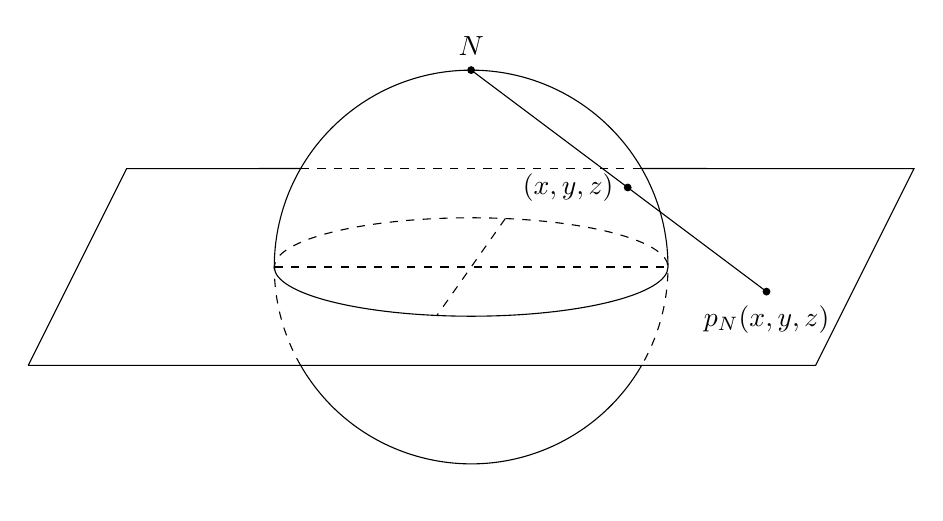
\begin{tikzpicture}[scale=1.25]
            \coordinate (A) at (3,-0.25);
            \coordinate (P) at (0,2);
      
            \draw (0:2cm)   arc[radius=2cm,start angle=0,end angle=180]
                  (210:2cm) arc[radius=2cm,start angle=210,end angle=330];
            \draw (180:2cm) arc[x radius=2cm, y radius=0.5cm, start angle=180,end angle=360];
      
            \draw [dashed] (210:2cm) 
                  arc[start angle=210,delta angle=-30,radius=2cm]
                  arc[start angle=180,delta angle=-180,x radius=2cm,y radius=0.5cm]
                  arc[start angle=0,delta angle=-30,radius=2cm];
      
            \draw [dashed] (80:2cm and 0.5cm) -- (260:2cm and 0.5cm);
            \draw [dashed] (150:2cm) coordinate(ul) -- (30:2cm) coordinate(ur);
      
            \draw (-4.5,-1) -- (3.5,-1) -- (4.5,1) -- (ur) (ul) -- (-3.5,1) -- (-4.5,-1);
      
            \draw (A) -- (P) coordinate[pos=0.47](B);
            \path (A) node[circle, fill, inner sep=1pt, label=below:{$ p_N(x,y,z) $}]{};
            \path (B) node[circle, fill, inner sep=1pt, label=left:{$ (x, y, z) $}]{};
            \path (P) node[circle, fill, inner sep=1pt, label=above:{$N$}]{};
            \draw [dashed] (-2,0) -- (2,0);
         \end{tikzpicture}
      \caption{Projection stéréographique de la sphère par rapport au pôle Nord}
   \end{figure*}
   On peut alors de manière analogue au cercle, trouver l'expression analytique des deux projections et montrer qu'elles munissent \( \mathbb{S}^2 \) d'une structure de variété différentielle.
\chapter{Espaces tangents dans \( \R^n \)}
   On aimerait alors pouvoir généraliser la notion \textbf{d'espace tangent} à une courbe, surface ... lisse de \( \R^n \) à des variétés abstraites comme définies dans les deux premiers chapitres. Pour ce faire, il est fondamental de comprendre que les variétés ainsi définies ne sont \textbf{pas} des objets de \( \R^k \), donc la notion de vecteur tangent géométrique perd son sens.\<

   L'approche fructueuse consiste alors à identifier \textbf{vecteurs} de \( \R^n \) et \textbf{dérivations} via la notion de dérivée directionnelle. On considère tout d'abord le cas de \( \R^n \), puis on généralise dans une variété quelconque.
   \section{Notion de dérivation:}
      Soit \(p \in \R^n\), on dira qu'un opérateur linéaire \( D: \mathcal{C}^\infty(\R^n) \longrightarrow \R \) est une \textbf{dérivation} en \( p \) si et seulement si il vérifie la règle de Leibniz:
      \[ 
         \forall f, g \in \mathcal{C}^\infty(\R^n) \; ; \; D(fg) = D(f)g(p) + f(p)D(g) 
      \]
      En particulier, les opérateurs de dérivées partielles d'une fonction lisse sont des dérivations. On peut aussi facilement montrer que si \( f \) est constante \( Df = 0 \) pour toute dérivation \( D \).
   \section{Espace tangent \( T\R^n_p \):}
      On appelle alors \textbf{espace tangent} à \( \R^n \) en \( p \) l'ensemble \( T\R^n_p \) de toutes les dérivations en \( p \) de fonctions lisses. On pose alors l'application suivante:
      \[ 
         \begin{aligned}
            \Phi : \R^n &\longrightarrow T\R^n_p \\
            v &\longmapsto \sum_{i \leq n} v_i \partialD{}{x_i}\biggr|_p
         \end{aligned} 
      \]
      Où les \( v_i \) sont les coordonées de \( v \) dans la base canonique. Alors on montre la propriété fondamentale qui est que \( \Phi \) est un \textbf{isomorphisme}. Ceci nous permet d'en déduire une base de \( T\R^n_p \) qui est alors donnée par:
      \[ 
         \Phi(e_i) = \partialD{}{x_i}\biggr|_p
      \] 
      Cette isomorphisme identifie donc les vecteurs et les dérivations. Les vecteurs ainsi définis agissent sur les fonctions lisses par dérivation directionelle, en effet si on considère par exemple:
      \[ 
         v = \partialD{}{x}\bigg|_{(x, y)} + 2\partialD{}{y}\bigg|_{(x, y)} \in T\R^n_{(x, y)}
      \] 
      Alors pour \( f(x, y) = xy \), on a:
      \[ 
         vf = \partialD{f}{x}(x, y) + 2\partialD{f}{y}(x, y) = y + 2x
      \]
\chapter{Espaces tangents sur une variété}
   On généralise l'approche du chapitre précédent au cas des variétés, et on en déduit une définition de l'espace tangent en un point. Dans toute la suite, on considèrera une fonction \( f : M \longrightarrow N \) point \( p \in M \), une carte \( \phi = (x_1, \ldots, x_n) \) et \( \psi = (y_1, \ldots, y_n) \) qui contiennent respectivement \( p \) et \( f(p) \)
   \section{Espace tangent en un point:}
      On définit une \textbf{dérivation} sur \( M \) en un point \( p \) comme un opérateur linéaire sur \( \mathcal{C}^\infty(M) \) qui vérifie la règle de Leibniz. On définit alors de manière analogue au cas euclidien \( TM_p \) comme l'ensemble des telles dérivations. C'est alors un espace vectoriel pour les lois usuelles.
   \section{Différentielle}
      On considère alors une application lisse \( f : M \longmapsto N \) et \( p \in M \). On définit alors la \textbf{différentielle} de l'application \( f \) en \( p \) par l'application suivante:
      \[ 
         \begin{aligned}
            df_p : TM_p &\longrightarrow TN_{f(p)} \\
            D &\longmapsto D(\cdot \circ f)
         \end{aligned} 
      \]
      C'est moralement une application qui transporte les dérivations. On peut alors vérifier que cette application est bien définie et qu'elle vérifie les propriétés suivantes:
      \begin{itemize}
         \item Elle est \textbf{linéaire}.
         \item Elle vérifie la \textbf{règle de la chaîne:} \( d(f \circ g)_p = df_{g(p)} \circ dg_p \)
         \item Si \( f \) est un \textbf{difféomorphisme}, alors \( df_p \) est un \textbf{isomorphisme}.
      \end{itemize}
   \section{Dimension et base}
   Alors en particulier si on considère une carte \( (U, \phi) \) qui contient \( p \), alors c'est un \textbf{difféomorphisme} et donc on a l'isomorphisme suivant:
      \[ 
         \begin{aligned}
            d\phi_p : TM_p &\longrightarrow T\R_{\phi(p)}^n
         \end{aligned} 
      \]
      On en déduis donc que \( TM_p \) est un espace vectoriel de dimension \( n \) et qu'une base  est donnée par:
      \[ 
         \partialD{}{x_i}\biggr|_p := d\phi_{p}^{-1}\left( \partialD{}{x_i}\biggr|_{\phi(p)}\right) 
      \]
      On verra dans la section suivante que ces vecteurs ont une action naturelle sur les fonctions lisses, similaire à celle dans \( \R^n \).
   \pagebreak
   \section{Action}
      Si \( f : M \longrightarrow \R \) est une fonction lisse, ces vecteurs de base agissent sur celle-ci par dérivation partielle dans les coordonées locales:
      \[ 
         \partialD{}{x_i}\biggr|_pf = \partialD{f \circ \phi^{-1}}{x_i}(\phi(p))
      \]
      Si \( f : M \longrightarrow N \), alors étant donnée une carte \( \psi \) sur \( N \), on définit les \textbf{composantes} \( f_j = (f \circ \psi)_j \) de \( f \) dans cette carte et ceci permet de définir une action de ces dérivées partielles sur \( f \) par:
      \[ 
         \partialD{}{x_i}\biggr|_pf := \left(\partialD{}{x_i}\biggr|_pf_1, \ldots, \partialD{}{x_i}\biggr|_pf_n\right)
      \]
   \section{Changement de représentation des vecteurs tangents}
      Dans la section précédente on a défini une représentation en coordonées locales d'un vecteur de l'espace tangent \( TM_p \), une question naturelle est alors:
      \begin{center}
         \textit{Quel est le lien entre deux telles représentations dans deux cartes différentes ?}
      \end{center}
      On peut alors montrer la propriété suivante si \( (U, \phi), (V, \psi) \) sont deux cartes qui contiennent un point \( p \), alors si on note \( x_i, y_i \) les coordonées respectives dans la première et la deuxième carte et \( c = \psi \circ \phi^{-1} \) l'application de changement de carte alors:
      \begin{align*}
         \partialD{}{x_i}\biggr|_p &= \sum_{j \leq n} \partialD{c_j}{x_i}(\phi(p)) \partialD{}{y_j}\biggr|_p
      \end{align*}
      On peut alors en déduire que la matrice de passage de la base en \( x_i \) vers celle en \( y_i \) est la jacobienne du changement de cartes.
   \section{Fibré tangent}
   On cherche alors a globaliser la notion d'espace tangent ponctuel et considérer \textbf{l'ensemble de tout les espaces tangents}. Ce point de vue est fructueux car il permettra de définir de manière simple la notion de champs de vecteurs sur une variété. On appelle cet ensemble le \textbf{fibré tangent} de \( M \) et il est défini par:
   \[ 
      TM = \bigsqcup_{p \in M} TM_p = \bigcup_{p \in M} \{p\} \times TM_p
   \]
   \begin{figure}[h]
      \centering
      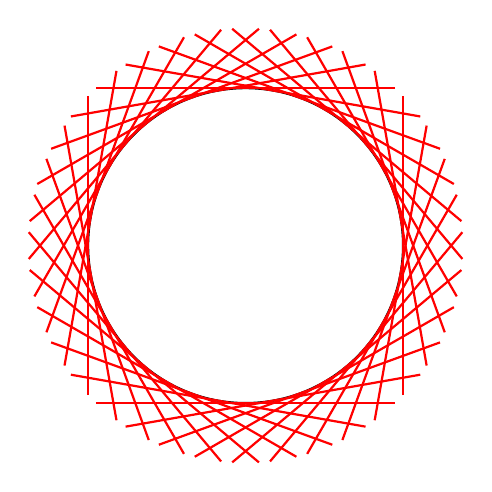
\begin{tikzpicture}
         % Dessiner le cercle
         \draw[thick] (0,0) circle (2);
         
         % Définir des points sur le cercle et leurs tangentes
         \foreach \angle in {10, 20, 30, 40, 50, 60, 70, 80, 90, 100, 110, 120, 130, 140, 150, 160, 170, 180, 190, 200, 210, 220, 230, 240, 250, 260, 270, 280, 290, 300, 310, 320, 330, 340, 350, 360} {
            % Calcul des coordonnées du point sur le cercle
            \pgfmathsetmacro\x{2*cos(\angle)}
            \pgfmathsetmacro\y{2*sin(\angle)}
            
            % Calcul du vecteur tangent (perpendiculaire au rayon)
            \pgfmathsetmacro\tx{-sin(\angle)}
            \pgfmathsetmacro\ty{cos(\angle)}
            
            % Tracer une droite tangentielle passant par le point
            \draw[red, thick] 
               ({\x - 1.9*\tx}, {\y - 1.9*\ty}) -- 
               ({\x + 1.9*\tx}, {\y + 1.9*\ty});
         }
      \end{tikzpicture}
      \caption{Fibré tangent du cercle \( \mathbb{S}^1 \)}
   \end{figure}

   Le fibré tangent hérite alors naturellement d'une projection \( \pi : (p, v) \in TM \mapsto p\) qui projete chaque vecteur sur son point base.
   \pagebreak
   \section{Structure du fibré tangent}
   De ces propriétés, on peut alors montrer que \( TM \) peut être muni d'une structure de \textbf{variété différentielle} de dimension \( 2n \). En effet on considère une carte \( (U, \phi) \) de \( M \), alors celle-ci induit l'application suivante:
   \begin{align*}
      \Phi : \pi^{-1}(U) &\longrightarrow \phi(U) \times T\R^{n}_p\\
      (p, v) &\longmapsto (\phi(p), d\phi_p(v))
   \end{align*}
   Alors cette application est bijective. L'atlas \( (U_\alpha, \phi_\alpha) \) induit donc une famille \((\pi^{-1}(U_\alpha), \Phi_\alpha)\) qui possède les propriétés suivantes:
   \begin{itemize}
      \item La famille des \(\Phi_\alpha \) induit une \textbf{topologie séparée} sur \( TM \).
      \item La famille des \(\Phi_\alpha \) est alors une famille \textbf{d'homéomorphismes} pour cette topologie.
      \item La famille des \( \pi^{-1}(U_\alpha) \) est un \textbf{recouvrement localement fini} de \( TM \).
   \end{itemize}
   Ceci munit \( TM \) d'une structure de variété topologique de dimension \( 2n \). En outre, on montre aussi que les changements de cartes sont lisses, et donc \( TM \) est muni d'une structure de variété différentielle.\<

   Un des intérêts de cette notion est qu'on peut alors identifier la différentielle comme une application globale sur les fibrés donnée par:
   \[ 
      \begin{aligned}
         df : TM &\longrightarrow TN \\
         (p, v) &\longmapsto (f(p), df_p(v))
      \end{aligned} 
   \]
   En fait, les cartes de \( TM \) s'identifient alors exactement aux différentielles globales des cartes de \( M \).
   \section{Champs de vecteurs}
   On peut alors définir la notion de \textbf{champs de vecteurs} sur une variété \( M \) par la donnée d'une application lisse de la forme:
   \[ 
      \begin{aligned}
         V : M &\longrightarrow TM \\
         p &\longmapsto (p, v)
      \end{aligned} 
   \]
   Où on identifiera \( V(p) \triangleq v \). Alors plus précisément, si on fixe \( p \in M \), alors en coordonées locales on a:
   \[ 
      V(p) = \sum_{i = 1}^n V_i(p) \partialD{}{x_i}\biggr|_p
   \]
   Un tel champs de vecteurs est dit lisse au sens d'une application lisse entre les variétés \( M \) et \( TM \), on note alors $\mathfrak{X}(M) $ l'ensemble des champs de vecteurs lisse sur \( M \). On peut caractériser le caractère lisse d'un tel champs par le caractère lisse de toutes ses composantes.
   \section{Opérations algébriques sur les champs de vecteurs}
      On peut alors définir les opérations algébriques usuelles sur les champs de vecteurs, notamment si \( X, Y \) sont deux champs de vecteurs et \( \lambda \in \R \), alors on définit:
      \[ 
         X + Y : p \in M \longmapsto (p, X_p + Y_p) \in TM \quad\quad \lambda X: p \in M \longmapsto (p, \lambda X_p) \in TM
      \]
      On peut aussi restreindre un champs de vecteurs lisse à une partie quelconque \( A \subseteq M \) en un champs de vecteurs lisse. Ceci vient directement du fait que la restriction d'une fonction lisse à une partie est lisse.
   \section{Pushforward d'un champs de vecteurs}
      Soit \( f : M \longrightarrow N \) une application lisse, l'utilité principale de la différentielle est de pouvoir transporter des vecteurs tangents à \( M \) sur des vecteurs tangents à \( N \), on peut alors se demander si on peut transporter un champs de vecteurs \( X : M \longrightarrow TM \) de la sorte, on peut toujours définir:
      \[ 
         g_X : p \in M \longmapsto (f(p), df_p(X_p)) \in TN
      \]
      Mais ce n'est pas à proprement parler un champs de vecteurs sur \( N \) du fait du domaine de définition, néanmoins si \( f \) est une \textbf{difféomorphisme}, on peut définir le \textbf{pushforward} de \( X \) induit par \( f \) par:
      \[ 
         f_*X : q \in N \longmapsto (q \; ; \; df_{f^{-1}(q)}(X_{f^{-1}(q)})) \in TN
      \]
      On obtient bien ainsi un champs de vecteurs sur \( N \).
\chapter{Espaces cotangents et puissances exterieures sur une variété}
   On peut alors considérer naturellement l'espace dual à l'espace tangent en un point \( p \in M \) et on définit ainsi \textbf{l'espace cotangent} en un point. On notera une base de cet espace, dans des coordonées locales, par la famille \( (dx_i)_{i \leq n} \) qui vérifie par définition pour la base associée à une carte fixée que:
   \[ 
      dx_i\left(\partialD{}{x_j}\biggr|_p\right) = \delta_{i, j}
   \]
   On peut alors considérer sa \( k \)-ième puissance extérieure \( \Lambda^k(TM_p^*) \) conformément au chapitre d'algèbre. On peut ainsi constuire des \textbf{tenseurs covariants antisymétriques} en un point de la variété. Etant donnée une carte locale, alors on peut définir une base de chacun de ces espaces de la même manière que dans le chapire d'algèbre et obtenir:
   \begin{itemize}
      \item Pour les vecteurs cotangents une expression de la forme \( \sum_{i \leq n} \omega_idx^i \).
      \item Pour les tenseurs covariants antisymétriques une expression de la forme \( \sum_{I} \omega_Idx^I \).
   \end{itemize}
   Aussi, par un résultat d'algébre linéaire élémentaire, la matrice de changement de base est alors donnée par la transposée de la matrice jacobienne.
   \section{Fibré cotangent}
      On cherche alors a globaliser la notion d'espace cotangent ponctuel et considérer \textbf{l'ensemble de tout les espaces cotangents}. Ce point de vue est fructueux car il permettra de définir de manière simple la notion de champs de covecteurs sur une variété. On appelle cet ensemble le \textbf{fibré cotangent} de \( M \) et il est défini par:
      \[ 
         TM^* = \bigsqcup_{p \in M} TM^*_p = \bigcup_{p \in M} \{p\} \times TM^*_p
      \]
      Aussi, il vérifie des propriétés analogues au fibré tangent, c'est aussi une variété de dimension \( 2n \). 
   \section{Fibré extérieur}
      On cherche alors a globaliser la notion d'espace extérieur ponctuel et considérer \textbf{l'ensemble de tout les espaces extérieurs}. Ce point de vue est fructueux car il permettra de définir de manière simple la notion de champs de tenseurs sur une variété. On appelle cet ensemble le \textbf{fibré extérieur} de \( M \) et il est défini par:
      \[ 
         \Lambda^k(TM^*) = \bigsqcup_{p \in M} \Lambda^k(TM_p^*) = \bigcup_{p \in M} \left\{ p \right\} \times \Lambda^k(TM_p^*) 
      \]
      Aussi, il vérifie des propriétés analogues aux précédents fibrés, c'est aussi une variété de dimension \( n + \binom{k}{n} \). 
   \section{Produit extérieur}
      On peut alors étendre la définition du produit extérieur aux tenseurs antisymétriques en un point de la variété et ce dernier respecte toutes les propriétés algébriques usuelles.
   \section{Différentielle abstraite et différentielle usuelle:}
      L'expression de la différentielle d'une fonction \( f : M \longrightarrow \R \) s'identifie à l'expression usuelle d'une différentielle, en effet, si \( v \in TM_p \), alors on peut montrer l'expression suivante:
      \[ 
         df_p(v) = \sum_{i=1}^n v_i \partialD{f}{x_i}(p)\partialD{}{t}\biggr|_{f(p)}
      \]
      Or, en faisant l'identification usuelle entre les dérivations est les vecteurs, on peut identifier cette expression à un vecteur de \(\R\) et on a aussi \( v_i = dx_i(v) \) donc on a l'identification naturelle suivante:
      \[ 
         df_p(v) \triangleq \sum_{i=1}^n \partialD{f}{x_i}(p)dx^i(v)
      \]
      On remarque alors que \( df_p \in TM^*_p \), on peut donc identifier la différentielle d'une fonction scalaire évaluée en un point à un vecteur cotangent, ie une forme linéaire sur l'espace tangent.\<

      Plus généralement, l'expression de la différentielle d'une fonction \( f : M \longrightarrow N \) s'identifie aussi à l'expression usuelle d'une différentielle, en effet, si \( v \in TM_p \), alors on trouve l'expression suivante:
      \[ 
         df_p(v) = \sum_{j=1}^m\sum_{i=1}^n v_i \partialD{f_j}{x_i}(p)\partialD{}{y_j}\biggr|_{f(p)}
      \]
      Or, en faisant l'identification usuelle entre les dérivations est les vecteurs, on peut identifier cette expression à un vecteur de \(\R^m\) et on a aussi \( v_i = dx_i(v) \) donc on a l'identification naturelle suivante:
      \[ 
         df_p(v) \triangleq (df_{1, p}(v), \ldots, df_{m, p}(v))
      \]
      De manière analogue on peut aussi remarque que la matrice de la différentielle dans les cartes est alors donnée par la jacobienne associée.
\chapter{Formes différentielles}
   On peut alors définir la notion de \textbf{champs de tenseurs contravariants} sur une variété \( M \), appelés \( k \)-formes différentielles et dont l'ensemble est noté \( \Omega^k(M) \). Elles sont définies par la donnée d'une application lisse de la forme:
   \[ 
      \begin{aligned}
         \omega : M &\longrightarrow \Lambda^kTM^* \\
         p &\longmapsto (p, \omega_p)
      \end{aligned} 
   \]
   Où on identifiera \( \omega(p) \) et \(\omega_p\). Alors plus précisément, si on fixe \( p \in M \), alors dans des coordonées locales autout de ce point, on a:
   \[ 
      \omega_p = \sum_I \omega_I(p) dx^I
   \]
   Une telle forme est dite lisse au sens d'une application lisse entre les variétés \( M \) et \( \Lambda^kTM^* \). On peut caractériser le caractère lisse d'une telle forme par le caractère lisse de toutes ses composantes (la preuve est la même que pour les champs de vecteurs).

   \section{Différentielle d'une fonction}
   On remarque alors qu'un exemple remarquable de 1-forme différentielle est celui de la différentielle elle même d'une fonction \( f : M \longrightarrow \R \), en effet, on a expliqué plus haut que l'on peut identifier:
   \[ 
      df_p \triangleq \sum_{i=1}^n \partialD{f}{x_i}(p)dx^i
   \]
   \section{Formes volumes}
      Le cas particulier des \(n\)-formes différentielles est fondamental, en effet soit \( \omega \) une telle forme, alors elle vérifie en coordonées locales:
      \[ 
         \omega_p =  f(p)dx^1 \wedge \ldots \wedge dx^n
      \]
      Si \( f \) ne s'annule jamais, on dira alors que \( \omega \) est une \textbf{forme volume}. Dans le cas particulier \( M = \R^n \), on peux alors identifier le déterminant canonique à la \( n \)-forme différentielle (constante) suivante:
      \[ 
         \omega(p) = dx^1 \wedge \ldots \wedge dx^n = \text{det}
      \]
      On a alors, par exemple:
      \begin{itemize}
         \item Dans \(\R^1\), on a \(\text{det} = dx\)
         \item Dans \(\R^3\) on a \(\text{det} = dx \wedge dy \wedge dz\)
      \end{itemize}
      En particulier, la formule du produit extérieur nous donne par exemple dans \(\R^2\) comme on l'attendrais intuitivement que:
      \[ 
         dx \wedge dy(u, v) = u_1v_2 - u_2v_1 = \text{det}(u, v)
      \]
   \section{Opérations algébriques sur les formes différentielles}
      On peut alors définir les opérations algébriques usuelles sur les formes différentielles, notamment si \( \omega, \eta \) sont deux formes différentielles de même degré et \( \lambda \in \R \), alors on définit:
      \[ 
         \omega + \eta : p \in M \longmapsto (p, \omega_p + \eta_p) \in \Lambda^kTM^* \quad\quad \lambda \omega: p \in M \longmapsto (p, \lambda \omega_p) \in \Lambda^kTM^*
      \] 
      On peut aussi restreindre une forme différentielle à une partie quelconque \( A \subseteq M \) en une forme différentielle lisse. Ceci vient directement du fait que la restriction d'une fonction lisse à une partie est lisse.
   \section{Evaluation d'un forme}
      Une 1-forme différentielle \( \omega \) étant un champs de formes linéaires, si on fixe \( p \in M \), on peut alors évaluer cette forme en un champs de vecteurs \( X \), et cette opération est donnée par:
      \[ 
         \omega(X) : p \longmapsto \omega_p(X_p)
      \]
      Alors, on peut exprimer cette évaluation en coordonées locales, ie si on a une 1-forme différentielle \( \omega \) et un champs de vecteurs \( X \) respectivement de la forme \( \omega = \sum_I \omega_I dx^I \) et \( X = \sum_i x_i \partialD{}{x_i}\big|_p\), on a directement par définition de la base duale:
      \begin{align*}
         \omega(X)(p) = \sum_{1 \leq i \leq n} \omega_{i}(p)x_i(p)
      \end{align*} 
      Donc on peut voir une 1-forme comme un objet qui prends un \textbf{champs de vecteurs} et retourne une \textbf{fonction}. De manière générale, on peut évaluer une \( k-\) forme sur \( k \) champs de vecteurs \( X_1, \ldots, X_k \) pour obtenir une fonction.
   \section{Produit extérieur des formes}
      Ponctuellement, on sait définir le produit extérieur de deux tenseurs covariants antisymétriques, on peut alors définir le produit extérieur de deux formes \( \omega, \eta \) d'ordre respectifs \( p, q \) par:
      \[ 
         \begin{aligned}
            \omega \wedge \eta : M &\longrightarrow \Lambda^{p+q}TM^* \\
            p &\longmapsto (p, \omega_p \wedge \eta_p)
         \end{aligned}
      \]
      Alors, il vérifie des propriétés analogues au produit extérieur classique, car il les vérifie en tout point. Notamment, il est bilinéaire alterné, et se réduit à la multiplication scalaire sur les 0-formes.
   \section{Pullback d'une forme}
   Dans la section sur les champs de vecteurs, on a vu que la différentielle d'une application \( f : M \longrightarrow N \) permet de transporter ceux-ci par \textbf{pushforward}. On définit ici le concept dual (associé à l'adjoint de la différentielle) qui permet de transporter des champs de covecteurs dans le sens opposé.\<

   Etant donnée une \( 1 \)-forme \( \omega \) sur \( N \), on peut alors \textbf{toujours} définir le \textbf{pullback} de \( \omega \) induit par \( f \) par:
   \[ 
      f^*\omega : p \in M \longrightarrow (p, \omega_{f(p)} \circ df_p) \in TM^*
   \]   
   De manière générale pour une \( k \)-forme on définit en composant par un \( k \)-uplet de différentielles de \( f \):
   \[ 
      f^*\omega : p \in M \longrightarrow (p, \omega_{f(p)} \circ (df_p, \ldots, df_p)) \in TM^*
   \]
   Alors ce sont bien des formes différentielles sur \( M \). 
   \pagebreak
   \section{Propriété du pullback}
      Le pullback sera fondamental dans la définition de l'intégrale sur une variété, on doit donc étudier ses nombreuses propriétés, en effet on peut montrer les propriétés suivantes:
      \begin{itemize}
         \item Le pullback est \textbf{linéaire}.
         \item Le pullback respecte le \textbf{produit extérieur}:
         \[ 
            f^*(\omega \wedge \eta) = f^*\omega \wedge f^*\eta
         \]
         \item Le pullback respecte la \textbf{différentielle} d'une fonction:
         \[ 
            f^*(dx) = d(f^*x)
         \]
      \end{itemize}
      Muni de ces propriétés on peut montrer pour une \( k-\)forme sur \( N \) que l'expression de son pullback en coordonées locales est donnée par:
      \[ 
         f^*\omega = \sum_{1 \leq i_1 < \ldots < i_k \leq n} (\omega_{i_1, \ldots, i_k} \circ f) df^{i_1} \wedge \ldots \wedge df^{i_k}
      \]
      En particulier, si \( \omega \) est \( n-\)forme sur \( N \) et que \( f \) est un \textbf{difféomorphisme}, on peut montrer la propriété fondamentale suivante qui n'est pas sans rapeller celle du changement de variables:
      \[ 
         f^*\omega = (\omega \circ f) \text{det}(\text{Jac}_f) dx^{1} \wedge \ldots \wedge dx^{n}
      \]
   \section{Dérivée extérieure}
      Un des outils principaux pour démontrer le théorème de Stokes est alors la généralisation de la notion de différentielle en un opérateur capable de différentier les \( k \)-formes. On appelle alors \textbf{dérivée extérieure} sur \( M \) la donnée pour tout \( k \in \N \) d'opérateurs linéaires de la forme:
      \[ 
         d_k : \Omega^k(M) \longrightarrow \Omega^{k+1}(M) 
      \]
      
      On note généralement simplement \( d \) tout ces opérateurs, en rendant implicites le degré des formes évaluées. On impose en outre les conditions supplémentaires suivantes à celui-ci:
      \begin{itemize}
         \item \textbf{Généralisation:} Si \( f \in \Omega^0(M)\), alors \( df \) correspond à la différentielle usuelle de \( f \).
         \item \textbf{Propriété fondamentale:} C'est un opérateur idempotent, ie \(d \circ d = 0\)
         \item \textbf{Propriété de Leibniz:} Si \( \omega \in \Omega^k(M) \) et \( \eta \in \Omega^l(M) \), alors on a:
         \[ 
            d(\omega \wedge \eta) = d\omega \wedge \eta + (-1)^k\omega \wedge d\eta 
         \]
      \end{itemize}
      On peut alors déduire de cette définition deux propriétés fondamentales:
      \begin{itemize}
         \item La propriété de Leibniz implique que c'est un \textbf{opérateur local}.
         \item La propriété de Leibniz implique que cet opérateur \textbf{commute avec le pullback}, ie:
         \[ 
            \forall \omega \in \Omega^k(M) \; ; \; f^*(d\omega) = d(f^*\omega)
         \]
      \end{itemize}
   \section{Existence de la dérivée extérieure}
      On cherche alors une forme nécessaire, pour toute forme \( \omega \in \Omega^k(M) \), si \( (U, \phi) \) est une carte, on a:
      \[ 
         d\omega|_U = \sum_I d\omega_I \wedge dx^I = \sum_I \sum_{j \leq n} \partialD{\omega_I}{x_j} dx^j \wedge dx^I
      \]
      Sur \( U \), il existe donc une unique dérivée extérieure définie par l'expression ci-dessus. On définit alors une dérivée extérieure \( d : \Omega^k(M) \longrightarrow \Omega^k(M) \) globalement par l'expression trouvée ci-dessus dans la carte \( (U, \phi) \), ie:
      \[ 
         d\omega_p = (d\omega|_U)_p
      \]
      
      On montre alors que cette définition ne dépends pas de la carte \( (U, \phi) \) choisie et que cet opérateur ainsi défini est \textbf{unique}.

\chapter{Orientation d'une variété}
   Dans le troisième chapitre, on a défini la notion de variété à bord, puis par la suite celle de forme volume qui définit si une variété est orientable ou non. On se pose alors les questions suivantes
   \begin{itemize}
      \item \textit{Si une variété est orientable, qu'est ce qu'une "orientation" de celle ci ?}
      \item \textit{Si une variété est orientable, est-ce que son bord l'est et comment l'orienter ?}
   \end{itemize}
   \section{Notion d'orientation}
      Soit \( M \) une variété orientable, alors on définit la relation d'équivalence suivante sur les formes volumes:
      \[ 
         \forall \omega, \omega' \in \Omega^n(M) \; , \; \omega \sim \omega' \iff \exists f > 0 \text{ telle que } \omega = f \cdot \omega' 
      \]
      On appelle \textbf{orientation} de \( M \) un choix d'une classe d'équivalence pour chaque composante connexe de \( M \). Dans une de ces composantes connexes, on montre qu'il n'y a que \textbf{deux classes d'équivalences}.

      Par exemple sur \( \R^3 \), voici deux représentants des deux classes d'équivalences:
      \[ 
         \text{det} = dx \wedge dy \wedge dz \quad\quad\quad \overline{\text{det}} = dy \wedge dx \wedge dz
      \]
      On note alors \( (M, \omega) \) une variété orientée par la forme volume \( \omega \). Si \( M \) est une variété orientée, ie telle qu'on a choisi une orientation sur celle-ci, on note \( -M \) la variété d'orientation opposée. 
   \section{Cas particulier des variétés de dimension nulle}
      Si \( M \) est de dimension nulle, alors c'est un ensemble fini de points, se pose alors la question suivante: 
      \begin{center}
         \textit{Que signifie alors une orientation sur une des composantes connexes (ie sur un point) ?}
      \end{center}
      C'est un fait simplement la donnée d'un signe \( \pm \) sur ce point, en effet une \( 0-\)forme est un nombre et donc une forme volume correspond ici à un nombre qui ne s'annule jamais.
   \section{Orientation de l'espace tangent}
   La donnée d'une orientation ainsi définie sur \( M \) et en fait exactement la donnée d'une même orientation sur chaque espace tangent. En particulier on dira qu'une base \( \mathcal{B} = (v_1, \ldots, v_n) \) de \( TM_p \) est \textbf{directe} si et seulement si:
   \[ 
      \omega_p(v_1, \ldots, v_n) > 0
   \]
   Aussi si on considère \( n \) champs de vecteurs \( X_1, \ldots, X_n \) tels qu'en tout points, ils forment une base de \( TM_p \), la fonction numérique suivante ne s'annule pas et est lisse:
   \[ 
      p \longmapsto \omega_p(X_1(p), \ldots, X_n(p)) 
   \]
   Donc en particulier, on peut faire en sorte qu'elle soit strictement positive, ie qu'elle munisse chaque espace tangent d'une base directe pour \( \omega\). Ceci donne une intérpretation géométrique simple à la notion d'orientabilité et d'orientation.
   \section{Difféomorphismes qui préservent l'orientation}
      On peut alors considérer deux variétés \( (M, \omega), (N, \eta) \) deux variétés orientées munies de leur atlas orienté. Alors on dira qu'un difféomorphisme \( F : M \longrightarrow N \) \textbf{respecte l'orientation} si et seulement si:
      \[ 
         F^*\eta \sim \omega
      \]
   \section{Atlas orienté}
      On considère dans toute la suite une variété orientable \( M \) muni d'une forme volume \( \omega \). On munit toujours \( \R^n \) de sa forme volume canonique, on définit alors la notion de \textbf{carte orientée} et on dira:
      \begin{itemize}
         \item Une carte est orientée \textbf{positivement} si elle préserve l'orientation de \( \R^n \), alors le coefficient de la forme volume est \textbf{positif}.
         \item Une carte est orientée \textbf{négativement} si elle ne préserve pas l'orientation de \( \R^n \), alors le coefficient de la forme volume est \textbf{négatif}.
      \end{itemize}
      On appelle alors \textbf{atlas orienté} un atlas tel que les cartes soient orientées positivement. Un résultat d'équivalence important (que nous ne démontrerons pas car inutile pour nous) est alors qu'une variété est orientable si et seulement si elle admet un atlas orienté.
   \section{Propriétés des atlas orientés}
      On peut montrer que si \( M \) est muni d'un atlas orienté, alors les changements de cartes ont un \textbf{jacobien positif}.\<
      
      En outre, si \( F : (M, \omega) \longrightarrow (N, \eta) \) est un difféomorphisme entre deux variétés orientées munis de tels atlas, on peut alors caractériser le fait qu'il préserve l'orientation par la positivité de son déterminant jacobien dans n'importe quelles cartes. 
   \section{Produit intérieur d'une forme}
         En effet, étant donné un champs de vecteurs \( X \), on peut construire une \( k-1 \) forme à partir d'une \( k \) forme par évaluation partielle en \( X \) sur la premier composante, cette opération apellée \textbf{produit intérieur} est définie par:
         \[ 
            \iota_X(\omega) : p \mapsto \omega(X_p, \cdot, \ldots, \cdot)
         \]
         Ceci se généralise et on peut alors construire une \( k-p \) forme avec la donnée de \( p \) champs de vecteurs.
   \section{Vecteurs entrants et sortants}
      Soit $M$ une variété à bords, $p$ un point du bord et $(U, \phi)$ une carte qui contient $p$, alors tout vecteur de $v = TM_p$ est de la forme:
      \[ 
         v = \sum_{i \leq n} v_i \frac{\partial}{\partial x_i}
      \]
      Alors on définit la notion de vecteur entrant et sortant:
      \begin{itemize}
         \item On dira que $v$ est \textbf{entrant} si et seulement si $v_n > 0$.
         \item On dira que $v$ est \textbf{sortant} si et seulement si $v_n < 0$. 
      \end{itemize}
      On cherche alors à définir un champs de vecteurs sortants lisse \( X \) sur le bord de \( M \), on peut alors montrer qu'un tel champ \textbf{existe toujours} et il nous permettra alors de définir l'orientation sur \( \partial M \).  
   \section{Orientation du bord d'une variété}
      Soit $M$ une variété orientable de forme volume $\omega$, $X$ un champs de vecteurs sortants lisse sur le bord de \( M \), alors on définit sur $\partial M$ la $n-1$ forme $\iota_X(\omega)$ et on montre que c'est bien une forme volume sur le bord. En particulier, on a la propriété fondamentale suivante:
      \begin{center}
         \textbf{Le bord d'une variété orientable à bord est orientable.}
      \end{center}
   \pagebreak
   \section{Expression de la forme volume induite}
      Si \( \omega \) est la forme volume sur \( M \), de coordonées locales:
      \[ 
         \omega = \widetilde{\omega} dx^1 \wedge \ldots \wedge dx^n 
      \]
      Alors \( \iota_{S}(\omega) \) est la forme volume sur \( \partial M \) et a pour expression locale:
      \[ 
         \iota_{S}(\omega) = \widetilde{\omega} (-1)^n dx^1 \wedge \ldots \wedge {dx^{n-1}}
      \]
      Par exemple sur \( \partial \mathbb{H}^2 \), on a la forme volume \( dx \), mais on remarque que sur \( \partial \mathbb{H}^3 \), on obtient plutôt \(dy \wedge dx\) qui est l'orientation opposée à celle de \( \R^2 \).
   \section{Exemples pratiques d'orientation du bord d'une variété}
      De manière plus concrète, on peut considérer quelques exemples usuels de variété à bord pour essayer de mieux comprendre comment s'oriente le bord d'une variété. Voici quelques exemples:
      \begin{figure}[htbp]
            \centering
            \begin{subfigure}{.3\textwidth}
               \centering
               \begin{tikzpicture}
                  \tikzset{%
                     my arrow1/.style={
                     postaction={decorate,decoration={
                     markings,
                     mark=between positions 0.15 and 0.95 step 0.15 with {\arrow[line width=1.5pt, color=red]{stealth}}}}
                     },
                  }
                  % Points d'extrémité
                  \def\xa{-2} % Point a
                  \def\ya{0}
                  \def\xb{2}  % Point b
                  \def\yb{0}
   
                  % Courbe paramétrée "quelconque" avec points de contrôle aléatoires
                  \draw[thick, smooth, my arrow1, postaction={decorate}] (\xa, \ya) 
                  .. controls (-1.5, 0.8) and (-1, -0.8) .. (-0.7, 0.5) 
                  .. controls (-0.4, 1.2) and (-0.2, -1) .. (0.6, 0.6) 
                  .. controls (1, 1.5) and (1.5, 1) .. (\xb, \yb);
   
                  % Points d'extrémité
                  \filldraw (\xa, \ya) circle (1pt) node[below] {$\color{red}-a$};
                  \filldraw (\xb, \yb) circle (1pt) node[below] {$\color{red}+b$};
               \end{tikzpicture}
               \caption*{(1) Cas d'une courbe}
            \end{subfigure}
            \centering
            \begin{subfigure}{.3\textwidth}
               \centering
               \begin{tikzpicture}
                  \tikzset{%
                     my arrow1/.style={
                     postaction={decorate,decoration={
                     markings,
                     mark=between positions 0 and 1 step 0.1 with {\arrow[line width=1.5pt, color=red]{stealth}}}}
                     },
                  }
                  % Paramètres
               \def\r{1} % Rayon du disque unité
   
               % Disque unité (cercle)
               \draw[thick, my arrow1, postaction={decorate}] (0,0) circle (\r cm);
               \draw[-stealth, red, thick] (0, 0) -- (0,0.5) node at (-0.3,0.35) {$\partial_2$};
               \draw[-stealth, red, thick] (0, 0) -- (0.5,0) node at (0.4,-0.275) {$\partial_1$};
   
               % Champ de vecteurs normal externe (radial)
               \foreach \angle in {0, 22.5, 45, 67.5, 90, 112.5, 135, 157.5, 180, 202.5, 225, 247.5, 270, 292.5, 315, 337.5} {
                  \draw[-stealth, draw opacity=0.4, thick] ({cos(\angle)*\r}, {sin(\angle)*\r}) -- ({cos(\angle)*1.5*\r}, {sin(\angle)*1.5*\r});
                }
               \end{tikzpicture}
               \caption*{(2) Cas du cercle}
            \end{subfigure}
            \centering
            \begin{subfigure}{0.3\textwidth}
               \centering
               \begin{tikzpicture}
                  \tikzset{%
                     my arrow1/.style={
                     postaction={decorate,decoration={
                     markings,
                     mark=between positions 0 and 1 step 0.175 with {\arrow[line width=1.5pt, color=red]{stealth}}}}
                     },
                     my arrow2/.style={
                     postaction={decorate,decoration={
                     markings,
                     mark=between positions 0 and 1 step 0.175 with {\arrowreversed[line width=1.5pt, color=red]{stealth}}}}
                     },
                  }
                  % Paramètres du cylindre
                  \def\r{1} % Rayon du cylindre
                  \def\h{3} % Hauteur du cylindre
   
                  % Bord supérieur (ellipse en perspective)
                  \draw[thick, my arrow2, postaction={decorate}] (0,\h) ellipse (\r cm and 0.3*\r cm);
                  % Bord inférieur (ellipse en perspective)
                  \draw[thick, my arrow1, postaction={decorate}] (0,0) ellipse (\r cm and 0.3*\r cm);
               
                  % Arêtes latérales reliant les bords
                  \draw[thick] (-\r,0) -- (-\r,\h);
                  \draw[thick] (\r,0) -- (\r,\h);
                
                  \draw[-stealth, red, thick] (0,1.5) -- (0,2) node at (-0.3,1.84) {$\partial_2$};
                  \draw[-stealth, red, thick] (0,1.5) -- (0.5,1.5) node at (0.4,1.2) {$\partial_1$};

                  % Vecteurs sortants sur le bord inférieur (vers le bas)
                  \foreach \angle in {0, 45, 90, 135, 180, 225, 270, 315} {
                     \pgfmathsetmacro\xpos{\r * cos(\angle)}
                     \pgfmathsetmacro\ypos{0.3 * \r * sin(\angle)}
                     \draw[-stealth, black, draw opacity=0.35, thick] (\xpos, \ypos) -- (\xpos, \ypos - 0.3);
                  }
                  % Vecteurs sortants sur le bord supérieur (vers le haut)
                  \foreach \angle in {0, 45, 90, 135, 180, 225, 270, 315} {
                     \pgfmathsetmacro\xpos{\r * cos(\angle)}
                     \pgfmathsetmacro\ypos{\h + 0.3 * \r * sin(\angle)}
                     \draw[-stealth, black, draw opacity=0.35, thick] (\xpos, \ypos) -- (\xpos, \ypos + 0.3);
                  }
               \end{tikzpicture}
               \caption*{(3) Cas du cylindre}
            \end{subfigure}      
      \end{figure}

      En fait on comprends alors que pour orienter le bord sachant une orientation sur l'intérieur, il suffit de placer le premier vecteur de la base de l'intérieur dans la même direction que le vecteur sortant et l'orientation du bord est alors l'ajout de vecteurs tels que la base complétée coincide avec la base de l'intérieur.
   \section{Cas de \( \partial\mathbb{H}^n \)}
      Comme vu précédent le cas de \( \partial\mathbb{H}^n \) est spécifique car sa forme volume induite est donnée par:
      \[ 
         \omega = (-1)^n dx^1 \wedge \ldots \wedge {dx^{n-1}}
      \]
      En particulier on remarque deux cas:
      \begin{itemize}
         \item Si \( n \) est \textbf{pair}, alors l'orientation de \( \partial\mathbb{H}^n \) est celle de \( \R^{n-1} \).
         \item Si \( n \) est \textbf{impair}, alors l'orientation de \( \partial\mathbb{H}^n \) est opposée à celle de \( \R^{n-1} \).
      \end{itemize}
      Avec les notations définies plus haut, on note donc \( \partial\mathbb{H}^n = \pm\R^{n-1} \) selon la parité de \( n \). Ceci signifie aussi que le difféomorphisme suivant préserve l'orientation ssi \( n \) est pair:
      \begin{align*}
         Id : (\R^{n-1}, \text{det}) \longrightarrow (\partial\mathbb{H}^n, \iota_{S}(\omega))
      \end{align*}
